%%%% 参考了https://www.wondercv.com/的模板

\documentclass[11pt]{article}

% disable indent globally
\setlength{\parindent}{0pt}
% some general improvements, defines the XeTeX logo
\usepackage{xltxtra}
% use hyperlink for email and url
\usepackage{hyperref}
\hypersetup{hidelinks}
\usepackage{url}
\urlstyle{tt}

\usepackage{xcolor}
%%%% 统一一种颜色,偏蓝色,用于section下划线和fontawesome,这颜色是从一个北航Logo上取的
\definecolor{CVBlue}{RGB}{23,110,191}

%%% \widthof[]{} 用于特殊对齐时用到
\usepackage{calc}

%%%% 利用tikz来定位照片和学校Logo
\usepackage{graphicx}
\usepackage{tikz}
\usetikzlibrary{calc}


% loading fonts
\usepackage{fontspec}
\usepackage{xeCJK}
\CJKsetecglue{} %% 取消中文与数字之间间隙

%%%%% 字体需要自己下载安装,注意版权问题,这两种字体应该比较好看,英文Helvetica,中文方正兰亭黑,也是有多种版本,自己试试哪些好看。参考了https://www.wondercv.com/的模板
%%%%% windows系统好像需要先安装字体,之后下面语句就够了
%Main document font
%\setmainfont[
%BoldFont = HelveticaNeueLTPro-Md.otf ,
%]{HelveticaNeueLTPro-Roman.otf}
%
%\setCJKmainfont[
%BoldFont=Pro_GB18030 DemiBold.otf,
%]{Pro_GB18030.otf}

%%%%% 字体需要自己下载安装,注意版权问题
%%%%% linux系统只需要字体路径就行了,如下
% % Main document font
%\setmainfont[
%    Path = Font/,
%  Extension = .otf ,
%  BoldFont = HelveticaNeueLTPro-Md.otf ,
%]{HelveticaNeueLTPro-Roman.otf}
%
%\setCJKmainfont[
%Path = Font/,
%  Extension = .otf ,
%BoldFont=Pro_GB18030 DemiBold.otf,
%]{Pro_GB18030.otf}

%%%%% 定义更漂亮的“C++”,参考https://tex.stackexchange.com/questions/4302/prettiest-way-to-typeset-c-cplusplus 
%%%%% 貌似跟具体字体大小有关,需要调下参数,我测试感觉下面的比较好看
\usepackage{relsize}
\usepackage{xspace}
\protected\def\Cpp{{C\nolinebreak[4]\hspace{-.05em}\raisebox{.28ex}{\relsize{-1}++}}\xspace} 

% use fontawesome
\usepackage{fontawesome}
%\newfontfamily{\FA}{[FontAwesome.otf]}

\usepackage[
	a4paper,
	left=1.2cm,
	right=1.2cm,
	top=2.5cm,
	bottom=2.5cm,
	nohead
]{geometry}

\renewcommand{\baselinestretch}{1.2} %定义行间距1.2

\usepackage{titlesec}
\usepackage{enumitem}
\setlist{noitemsep} % removes spacing from items but leaves space around the whole list
%\setlist{nosep} % removes all vertical spacing within and around the list
\setlist[itemize]{topsep=0.25em, leftmargin=*}
\setlist[enumerate]{topsep=0.25em, leftmargin=*}



\titleformat{\section}         % Customise the \section command 
  {\large\bfseries\raggedright} % Make the \section headers large (\Large),
                               % small capitals (\scshape) and left aligned (\raggedright)
  {}{0em}                      % Can be used to give a prefix to all sections, like 'Section ...'
  {}                           % Can be used to insert code before the heading
  [{\color{CVBlue}\titlerule}]                 % Inserts a horizontal line after the heading
\titlespacing*{\section}{0cm}{*1.6}{*1.2}



\begin{document}
\pagenumbering{gobble} % suppress displaying page number

%%%% 利用tikz来定位照片,部分招聘单位可能需要“以貌取人”
\begin{tikzpicture}[remember picture, overlay] 
  \node[anchor = north east] at ($(current page.north east)+(-1cm,-1.5cm)$) {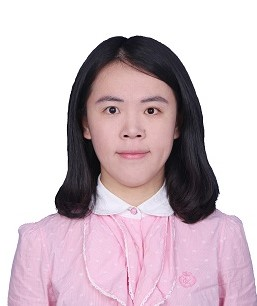
\includegraphics[height=2.5cm]{avatarWhite}};
\end{tikzpicture}%
%%%% 利用tikz来定位学校Logo,这里只在第一页显示,如果需要每页都有,可以考虑在页眉、页脚或者background中加入,不过简历也就一两页,无所谓了
%\begin{tikzpicture}[remember picture, overlay] 
%  \node[anchor = north west] at ($(current page.north west)+(0.2cm,-0.2cm)$) {\includegraphics[height=2cm]{buaa-markname-blue}};
%\end{tikzpicture}%
%%%% 利用tikz来定位页脚栏,电子版简历使用,黑白纸质打印效果可能并不好。这里只在第一页显示,如果需要每页都有,页脚或者background中加入。
%\begin{tikzpicture}[remember picture, overlay] 
%  \node[anchor = south,fill=CVBlue,draw=none,minimum width=\paperwidth,minimum height=1.5em,align=center,font=\footnotesize,text=white] at ($(current page.south)$) {\faLinkedinSquare \ https://www.linkedin.com/in/username \qquad \faGithub \ https://github.com/username \qquad \faRssSquare \ http://blog.yours.me};
%\end{tikzpicture}%
%tikzpicture环境很敏感,注释周围的空格、空行都会引起水平距离或垂直距离的变化,
%
\centerline{\LARGE\bfseries{王天天}}

\centerline{\normalsize{2021届博士生,研究方向:运筹优化、港口调度优化}}

\centerline{\normalsize{\faPhone\ 187-5858-2334 \quad \faEnvelopeO\ \href{mailto:wangtiantianzju@foxmail.com}{:wangtiantianzju@foxmail.com}}}


\section{\makebox[\widthof{\faGraduationCap}][c]{\color{CVBlue}\faGraduationCap}\  教育背景}

\textbf{浙江大学} \hfill 2013年 -- \makebox[\widthof{2013年}][s]{现在}

博士研究生\quad 管理科学与工程

\textbf{香港理工大学} \hfill 2016年 -- \makebox[\widthof{2016年}][s]{现在}

博士研究生\quad 物流与航运研究

\textbf{山东大学} \hfill 2009年 -- 2013年

理学学士\quad 数学-信息与计算科学

\section{\makebox[\widthof{\faGraduationCap}][c]{\color{CVBlue}\faUsers}\ 项目/实习经历}

\textbf{立库穿梭车取箱调度优化}\  \hfill 2020年6月 -- 2020年7月

实习\quad 菜鸟网络

针对多层穿梭车立体仓库,对其中货箱的出库问题建模,决策穿梭车和提升机资源的调度顺序,缩短出库时间。

\begin{itemize}
  \item 考虑有无缓存、不同深位大小的立库,建立多个不同的MIP模型;
  \item 用CPLEX求解,同时设计启发式算法求解;
  \item 模型效果比启发式方法稳定,处理50个货箱取出任务仍具有高效率,模型精确解超出启发式方法的解约30\%。
\end{itemize}

\textbf{货到人AGV调度优化}\  \hfill 2020年7月 -- 2020年8月

实习\quad 菜鸟网络

仓库内,移动式货柜由AGV托运依次访问多个拣选工作站。根据访问优先级,决策每个AGV访问各工作站的次序,以避免不同AGV之间的失控冲突,最小化访问成本。

\begin{itemize}
  \item 建立IP模型,并用Brach and price求解。
\end{itemize}

\textbf{带资源约束的服务网络设计}\  \hfill 2017年3月 -- 2017年6月

项目成员\quad 菜鸟网络

研究全国范围内干线物流的服务网络设计,设计模型和算法解决有货物-车辆资源匹配的路径优化问题。

\begin{itemize}
  \item 在缩减问题规模的基础上,用Branch and price以及启发式算法求解。
\end{itemize}


\section{\makebox[\widthof{\faGraduationCap}][c]{\color{CVBlue}\faLightbulbO}\ 研究经历}
\textbf{堆场集装箱存储空间动态分配优化}\  \hfill 2015年10月 -- 2017年2月

考虑存储空间根据时间动态利用释放的特征,从operational level对到港集装箱的存储位置进行精确到单位集装箱的空间分配计划,建模并设计算法提高空间利用率。

\begin{itemize}
  \item 建立了整数规划IP模型;
  \item 采用动态规划算法生成可行存储方法,然后在此基础上用贪心策略选择空间利用率最高的存储方案;
  \item 采用多种元启发式方式迭代需求调度次序;根据需求的时空间的特点设计了算法加速策略。
%,在小规模测试中用CPLEX求得最优解;
%  \item 贡献:目前主流的集装箱分配研究多集中在tactical level,本研究是为数不多的从operational level对存储空间分配的研究,充分考虑了存储空间被动态占用释放的难点;建立了整数规划MIP数学模型,在小规模测试中用CPLEX求得最优解;估计了问题的lower bound,求得存储方案与下界的gap较现有其他方法平均提高30\%。
%  \item 已经投稿到COR(第一作者)。
\end{itemize}

\textbf{考虑设备操作安全距离及负载均衡的集装箱空间分配优化}\  \hfill 2017年10月 -- 2018年9月

在集装箱存储空间分配问题中,对于单个箱区包含两个不可交叉通过的场桥(yard crane)情况,本研究在考虑场桥的安全距离、均衡多个场桥工作量的约束下动态分配存储空间。
\begin{itemize}
  \item 要求两个yard crane每时每刻都保持安全距离;
  \item 建立数学模型;设计启发式策略求解,本研究设计两阶段迭代算法求解。
%考虑单个箱区两个不可交叉通过的场桥,场桥的工作量同时包含集装箱装卸两种操作;设计两阶段迭代算法,第一阶段对每个场桥分配需要操作的集装箱(即来自各需求的集装箱数);第二阶段对所分配集装箱设计存储空间,判断计划存储空间是否满足场桥运行安全距离,若不满足则调整各场桥工作量。
\end{itemize}

\textbf{港口装卸设备调度及车辆路径设计综合优化}\  \hfill 2018年10月 -- 2019年11月

对港口集装箱转运过程涉及到的泊位分配、堆场存储空间分配、集卡路径进行综合优化。
\begin{itemize}
  \item 涉及模块:进出港轮船停泊位置分配,轮船所需岸桥(quay crane)分配,集装箱堆场存储位置分配,集卡往来泊位与堆场路线分配。
  \item 启发式算法,column generation(工作中)。
\end{itemize}



\section{\makebox[\widthof{\faGraduationCap}][c]{\color{CVBlue}\faBookmarkO}\ 论文}
% increase linespacing [parsep=0.5ex]
\begin{itemize}[parsep=0.5ex]
	\item \textbf{Tiantian Wang}, Hong Ma, Zhou Xu, Jun Xia. A New Dynamic Shape Adjustment and Placement Algorithm for the 3D Yard Allocation Problem with Time Dimension. Computers \& Operations Research, Under review.
	\item \textbf{Tiantian Wang}, Jun Xia. The integrated scheduling of yard space and yard cranes considering safety distance. Transportation Research Part E, Submitting.
\end{itemize}

\section{\makebox[\widthof{\faGraduationCap}][c]{\color{CVBlue}\faBook}\ 主要课程}
% increase linespacing [parsep=0.5ex]
\begin{itemize}[parsep=0.5ex]
  \item 运筹学,整数规划,离散优化,非线性规划,凸优化,随机模型,博弈论
  \item 数学分析,高等代数,概率论,数理统计,数值计算,控制论,算法,数据结构
\end{itemize}

\section{\makebox[\widthof{\faGraduationCap}][c]{\color{CVBlue}\faCogs}\ IT 技能}
% increase linespacing [parsep=0.5ex]
\begin{itemize}[parsep=0.5ex]
  \item 语言: Java(主要), Python, \Cpp, C
  \item 求解器: CPLEX
  \item 统计: Minitab, SPSS, Python
  \item Linux, Git
\end{itemize}


\section{\makebox[\widthof{\faGraduationCap}][c]{\color{CVBlue}\faLanguage}\ 英语水平}
\begin{itemize}[parsep=0.5ex]
  \item TOEFL 90
  \item GMAT 620
\end{itemize}

\section{\makebox[\widthof{\faGraduationCap}][c]{\color{CVBlue}\faInfo}\ 学术活动}
%\faInfo
% increase linespacing [parsep=0.5ex]
\begin{itemize}[parsep=0.5ex]
	\item 参加International Symposium on Scheduling 2017,并汇报。
	\item 参加第十四届物流系统工程学术研讨会,并汇报。
	\item 参加第12届运营管理与应急管理学术研讨工作坊,并汇报。
\end{itemize}

%%%% 如果多页简历,可以手动在适当位置插入 \newpage 或者 \clearpage 开始新一页

\end{document}
